%%%%%%%%%%%%%%%%%%%%%%%%%%%%%%%%%%%%%%%%%%%%%%%%%%%%%%%%%%%%%%%%%%%%%%%%%%%%%%%%
% Memoria para trabajos y entregas de laboratorio de la Escuela Superior de    %
% Informática (ESI) de Ciudad Real, UCLM.                                      %
%   Versión: Octubre - 2018                                                    %
%   Desarrollada por José Ángel Martín Baos                                    %
%                                                                              %
% Recursos:			                                                           %
%   - Contenidos del curso “LaTeX esencial para preparación de Trabajo Fin de  %
%     Grado, Tesis y otros documentos académicos” impartido por el profesor    %
%     Jesús Salido.                                                            %
%                                                                              %
% Disponible en: https://github.com/JoseAngelMartinB/PlantillaTrabajosLaTeX    %
%%%%%%%%%%%%%%%%%%%%%%%%%%%%%%%%%%%%%%%%%%%%%%%%%%%%%%%%%%%%%%%%%%%%%%%%%%%%%%%%

\documentclass[11pt]{article}

% PAQUETES USADOS:
\usepackage{natbib}
\usepackage{url}
\usepackage[utf8]{inputenc} % Codificación (Permite carácteres españoles)
\usepackage{amsmath}
\usepackage{graphicx}
\graphicspath{{images/}} % Carpeta en la cual se van a buscar las imagenes
\usepackage{subfigure}	% Permite la Inclusión de subfiguras
%\usepackage{parskip} % Suprime la identación de los parrafos.
\setlength{\parskip}{3mm} % Longitud del espaciado entre parrafos
\usepackage[hidelinks]{hyperref} % Referencias (links)
\usepackage{fancyhdr}
\usepackage{vmargin}
\usepackage{paralist} % Permite un mayor control sobre las listas
\usepackage{textcomp,marvosym,pifont} % Generación de símbolos especiales
\usepackage[usenames,dvipsnames,svgnames,x11names,table]{xcolor}
\usepackage{enumerate}

% CONFIGURACIÓN DE LA PÁGINA:
\setpapersize{A4} % Formato del papel - A4
\setmarginsrb{3 cm}{2.5 cm}{3 cm}{2.5 cm}{1 cm}{1.5 cm}{1 cm}{1.5 cm} % Margenes

% Complemento para insertar código en la memoria:
%   Basado en 'Listados de código cómodos y resultones con listings'
%   de David Villa en http://crysol.org/es/node/909
\usepackage{color}
\definecolor{gray97}{gray}{.97}
\definecolor{gray75}{gray}{.75}
\definecolor{gray45}{gray}{.45}
\usepackage{listings}
\lstset{ frame=Ltb,
	framerule=0pt,
	aboveskip=0.5cm,
	framextopmargin=3pt,
	framexbottommargin=3pt,
	framexleftmargin=0.4cm,
	framesep=0pt,
	rulesep=.4pt,
	backgroundcolor=\color{gray97},
	rulesepcolor=\color{black},
	texcl=true,
	%
	stringstyle=\ttfamily,
	showstringspaces = false,
	basicstyle=\small\ttfamily,
	commentstyle=\color{gray45},
	keywordstyle=\bfseries,
	%
	numbers=left,
	numbersep=15pt,
	numberstyle=\tiny,
	numberfirstline = false,
	breaklines=true,
}
% Minimizar fragmentado de listados
\lstnewenvironment{listing}[1][]
{\lstset{#1}\pagebreak[0]}{\pagebreak[0]}

\lstdefinestyle{consola}
{basicstyle=\scriptsize\bf\ttfamily,
	backgroundcolor=\color{gray75},
}

\lstdefinestyle{C}
{language=C,
}

%OTROS PAQUETES:
\usepackage{float} % Permite usar H en las figuras, de manera que se coloquen en la posición exacta en la que están en el código.

% Añade un comando para crear indicaciones de pulsación de teclas
\usepackage{tikz} % Paquete especializado en gráficos
\usetikzlibrary{shadows} % Necesario para poder crear nuevo comando de indicación de pulsación de tecla.
\newcommand*\tecla[1]{%
	\tikz[baseline=(key.base)]
	\node[%
	draw,
	fill=white,
	drop shadow={shadow xshift=0.25ex,shadow yshift=-0.25ex,fill=black,opacity=0.75},
	rectangle,
	rounded corners=2pt,
	inner sep=1pt,
	line width=0.5pt,
	font=\scriptsize\sffamily
	](key) {#1\strut}
	;
}

\newif\ifspanish % Condicional que permite seleccionar el lenguage.
\newif\ifmultipleauthors % Condicional que permite multiples autores
\spanishtrue
\multipleauthorsfalse


%%%%%%%%%%%%%%%%%%%%%%%%%%%%%%%%%%%%%%%%%%%%%%%%%%%%%%%%%%%%%%%%%%%%%%%%%%%%%%%%
%%%%%%%%%				Principales variables del documento			   %%%%%%%%%

\title{Práctica 2: Renderizado Gráfico}							% Titulo
\author{David Camuñas Sánchez}							% Autor

\date{18 de marzo de 2020}											% Fecha
\newcommand{\subject}{Diseño de Infraestructuras de Red}						% Asignatura
\newcommand{\course}{Grado en Ingeniería Informática}	% Curso
%\newcommand{\course}{Máster Universitario en Ingeniería Informática}	% Curso
\newcommand{\courseyear}{2019 - 2020} 					% Curso académico
%\spanishfalse	    	% Descomentar esta línea si el trabajo está en inglés
%\multipleauthorstrue   % Descomentar esta línea si hay varios autores

%%%%%%%%%%%%%%%%%%%%%%%%%%%%%%%%%%%%%%%%%%%%%%%%%%%%%%%%%%%%%%%%%%%%%%%%%%%%%%%%

\ifspanish
	\usepackage[spanish]{babel} % Paquete de español
	\newcommand{\dateText}{Fecha:}
	\renewcommand{\lstlistingname}{Listado} % Renombrar listados para que aparezcan en español.
	% Algoritmos
	\usepackage[ruled,vlined,spanish]{algorithm2e} % Permite pseudocódigos. NECESARIO INSTALAR texlive-science (sudo apt-get install texlive-science)
\else
	\usepackage[english]{babel} % Paquete de inglés
	\newcommand{\dateText}{Date:}
	% Algoritmos
	\usepackage[ruled,vlined,english]{algorithm2e}
\fi

\makeatletter
\let\thetitle\@title
\let\theauthor\@author
\let\thedate\@date
\makeatother

% Formato de página:
\pagestyle{fancy}		% Formato por defecto - Recomendado
%\pagestyle{headings} 	% Formato para libros
\fancyhf{}
\ifmultipleauthors
	\chead{\thetitle}
\else
	\rhead{\subject}
	\lhead{\thetitle}
\fi
\cfoot{\thepage}

\begin{document}

%%%%%%%%%%%%%%%%%%%%%%%%%%%%%%%%%%%%%%%%%%%%%%%%%%%%%%%%%%%%%%%%%%%%%%%%%%%%%%%%
%%%%%%%%							Portada							   %%%%%%%%%

\begin{titlepage}
	\centering
	\begin{minipage}[t]{\textwidth}
		\raisebox{-0.5\height}{
\includegraphics[scale = 0.5]{uclm.jpg}} 	% Logo de la universidad
		\hspace{\fill}
		\raisebox{-0.5\height}{
\includegraphics[scale = 0.5]{open-mpi.png}} 	% Logo de open-mpi
	\end{minipage}
	\\[2.25 cm]
    \textsc{\LARGE Universidad de Castilla-La Mancha}\\[1 cm]	% Nombre de la universidad
    \textsc{\LARGE Escuela Superior de Informática}\\[2.0 cm]
	\textsc{\Large \subject}\\[0.5 cm]				% Asignatura
	\textsc{\large \course \\ \courseyear}\\[2 cm]				% Curso
	\rule{\linewidth}{0.2 mm} \\[0.4 cm]
	{ \huge \bfseries \thetitle}\\
	\rule{\linewidth}{0.2 mm} \\[2.5 cm]

	\vspace*{\fill}
	\begin{minipage}{0.4\textwidth}
		\begin{flushleft} \large
			\ifspanish
				\ifmultipleauthors
					\emph{Autores:}\\
				\else
					\emph{Autor:}\\
				\fi
			\else
				\ifmultipleauthors
					\emph{Authors:}\\
				\else
					\emph{Author:}\\
				\fi
			\fi
			\theauthor
			\end{flushleft}
			\end{minipage}~
			\begin{minipage}{0.4\textwidth}
			\begin{flushright} \large
			\emph{\dateText} \\
			\thedate
		\end{flushright}
	\end{minipage}\\[2.25 cm]


\end{titlepage}

%%%%%%%%%%%%%%%%%%%%%%%%%%%%%%%%%%%%%%%%%%%%%%%%%%%%%%%%%%%%%%%%%%%%%%%%%%%%%%%%
%%%%%%%%%						   	Índice					      	   %%%%%%%%%

\tableofcontents
\pagebreak


%%%%%%%%%%%%%%%%%%%%%%%%%%%%%%%%%%%%%%%%%%%%%%%%%%%%%%%%%%%%%%%%%%%%%%%%%%%%%%%%
%%%%%%%%%							Documento						   %%%%%%%%%
\section{Enunciado}
Utilizaremos las primitivas pertinentes \textbf{\textit{MPI2}} como acceso paralelo a disco y
gestión de procesos dinámico:\\
Inicialmente el usuario lanzará un solo proceso mediante \textit{mpirun -np 1
./pract2}. Con ello MPI lanza un primer proceso que será el que tiene acceso a
la pantalla de gráficos pero no a disco. Él mismo será el encargado de levantar
N procesos (con N definido en tiempo de compilación como una constante) que
tendrán acceso a disco pero no a gráficos directamente.

Los nuevos procesos lanzados se encargarán de leer de forma paralela
los datos del archivo foto.dat. Después, se encargarán de ir enviando los pixels
al primer elemento de proceso para que éste se encargue de representarlo en
pantalla.

Usaremos la plantilla pract2.c para comenzar a desarrollar la práctica.
En ella debemos completar el código que ejecuta el proceso con acceso a la
ventana de gráficos (rank 0 inicial) y la de los procesos “trabajadores”.
Se proporciona el archivo foto.dat. La estructura interna de este archivo
es 400 filas por 400 columnas de puntos.\\
Cada punto está formado por una
tripleta de tres “unsigned char” correspondiendo al valor R,G y B de cada uno
de los colores primarios. Estos valores se pueden usar para la función
\textit{dibujaPunto}().

\newpage
% Sección: Intruducción
\section{Introducción}
El objetivo de esta práctica es la creación de un programa de rendrerizado gráfico, mediante el uso de las \textit{funciones} que nos ofrece \textbf{\textit{MPI}}.

A la hora de analizar una imagen, en este caso foto.dat, se puede tratar como si fuese una matriz de \textit{X} (filas) por \textit{Y} (columnas) dimensiones. En este caso, se trata de una matriz cuadrada de \textit{400 píxeles}, es decir, donde tanto el valor de las \textbf{filas} y \textbf{columnas} es de \textbf{400}. Por tanto el número total de pixeles que forman la matriz, es \textbf{$400^2$} \textit{($L^2$)} = \textbf{160000 píxeles}.\\
Estos valores estan indicados en el programa, en forma de constantes, en concreto, en el archivo \textit{include/definitions.h}.\\

En la Figura \ref{fig:intro}, se puede observar la estructura de una imagen junto con la imagen a renderizar. Donde cada píxel está formado por una
tripleta de tres parámetros de tipo “\textit{unsigned char}” correspondiendo al valor R,G y B de cada uno de los \textit{colores primarios}.

\begin{figure}[H]
  \centering
  \subfigure[Pixeles de una imagen]{
    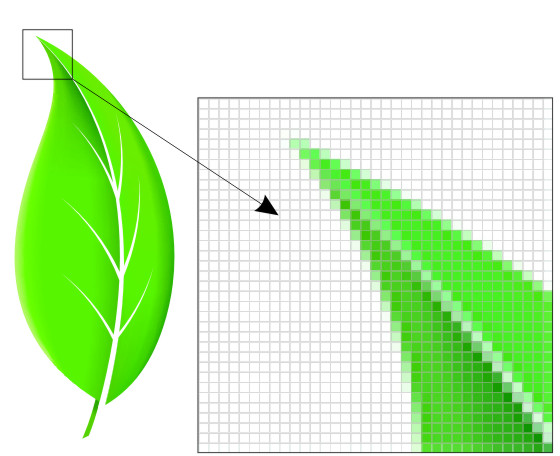
\includegraphics[width=70mm]{pixeles.jpg}
  }
  \subfigure[Imagen a renderizar]{
  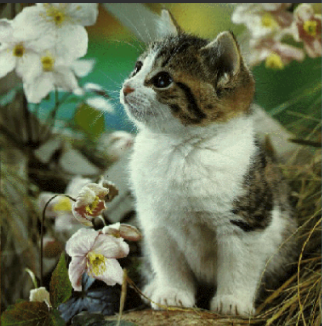
\includegraphics[width=50mm]{cat.png}
  
  }
  \caption{Representación de píxeles que forman una imagen}
  \label{fig:intro}
\end{figure}

\clearpage


\section{Planteamiento de la solución}
El programa comienza con a creación de un solo proceso, este proceso es el proceso principal, el cual corresponde al proceso cuyo \textit{RANK} es igual a 0. También conocido a lo largo del programa como el proceso \textbf{\textit{maestro}}.\\
Una vez lanzado el proceso \textit{maestro}, este creará una ventana gráfica haciendo uso de la librería \textit{\textbf{lX11}} (función \textit{initX()}). Además también creará \textbf{N} procesos hijos, conocidos a lo largo del programa como \textit{\textbf{esclavos o trabajadores}} (definidos con la constante creada eb tiempo de compilación \textit{EMPLOYEES-NUMBER}).\\

Tras lanzar el \textit{\textbf{maestro}} los N trabajadores, este se maltendra a la espera en todo momento, para recibir los pixeles de cada trabajador, los cuales debe de dibujar en la imagen.\\
Mientras el maestro se mantiene en dicha espera, a cada \textit{\textbf{trabajador}}, se le asignara una zona de trabaja, esta zona pertenece a un rango de lineas del fichero, el cual será obtenido de dividir el número de filas del fichero entre los trabajadores generados (el resto de la operación, si es que lo hubiese, será asignado al último trabajador, es decir al \textit{RANK} N-1).


\subsection{Tipos de nodos}
En este problema encontramos dos tipos de nodos: el \textbf{\textit{rank o nodo 0}} y los demás \textbf{\textit{nodos}}.

\begin{itemize}
	\item \textbf{Rank 0}: Este nodo corresponde al primer proceso creado. Encargado de la lectura del fichero \textit{\textbf{datos.dat}}, el cual contiene los números que más tarde asignara el mismo a los demás nodos que forman la red toroidal.
	
	A la hora de realizar la asignación de los números a los respectivos nodos restantes (incluyendose el mismo), debe de comprobar que la cantidad de números obtenidos del fichero es igual al tamaño del toroide \textbf{N} (nº de nodos que lo forman) si esta comprobación es exitosa, continuara la ejecución normal del programa.
	
	En caso contrario, a mi elección bien sea por que el tamaño del toroide o la cantidad de los números sea menor o mayor. El \textit{rank 0} cero abortará la ejecución del programa. 
	Tanto si la comprobación es correcta como si no, este difundirá el resultado a los demás nodos. Para ello se ha utilizado la función \textit{Bcast()} de la libreria de \textbf{MPI}.
	
	Una vez asignados los respectivos números a cada nodo, tras calcular el número mínimo de la red toroidal, \textit{rank 0} mostrara dicho número por pantalla, y el programa finalizará.
	
	\item \textbf{Los demás nodos}: Estos tipos de nodos recibirán del \textit{rank 0} la decisión de continuar o no. Si continua la ejecución normal se les asignará un número real, el cual trás obtener cada uno sus respectivos vecinos, se  llevará a cabo el algoritmo para obtener \textit{el menor número de la red toroidal}.
\end{itemize}


\subsection{Algoritmos principales}
Los algoritmos principales de esta práctica son: \textbf{la obtención de los vecinos} (de cada nodo) y \textbf{cálculo del número mínimo} de la red toroidal.

\subsubsection{Obtención de los vecinos}
Este algoritmo es fundamental en el programa, debido a que gracias a el se ve de una manera más intutiva la estructura de la red toroidal, donde cada nodo o rank conoce a sus respectivos vecinos. Cada nodo tiene un total de \textit{cuatro vecinos}, denominados: \textbf{Norte, Sur, Este y Oeste}.

En concreto los vecinos Norte y Sur de cada nodo, se han obtenido gracias al uso de las filas de la red toroidal. En cambio los vecinos Este y Oeste, se han obtenido gracias a las columnas.

Para saber en que posición se encuentra cada nodo o rank, dentro de la red toroidal, representada como una matriz de \textbf{LxL}. Que esta determinada por el número de fila y de columna \textbf{(fila,columna)}, por ejemplo: (0,0), (0,1), (1,0), etc.
Para determinar el valor de la fila, se ha utilizado la división de \textbf{L} entre el \textbf{rank} \cite{mpi_rank} del nodo actual (\textbf{L/rank}). Y para obtener el valor de la columna se hace al igual que la fila, pero en este caso con el módulo (\textbf{L\%rank}).

\begin{figure}[H]
  \centering
    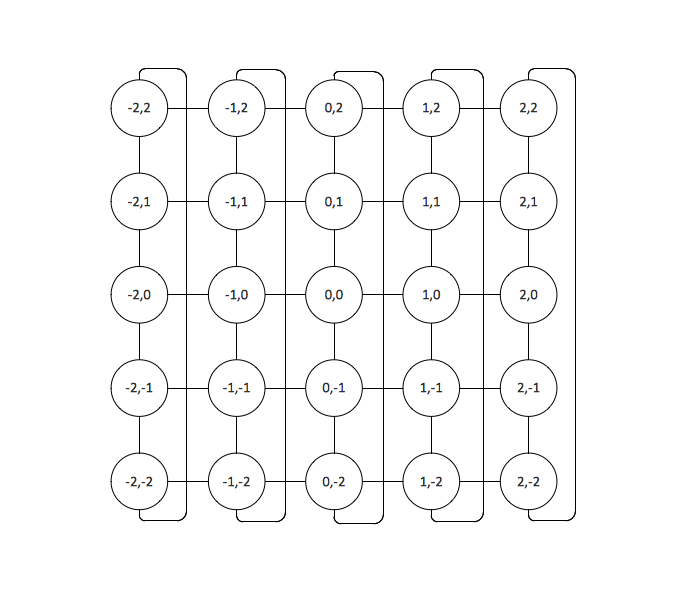
\includegraphics[width=65mm]{matriz.png}
  \caption{Representación red toroidal como una matriz.}
  \label{fig:matriz}
\end{figure}


\begin{itemize}
	\item \textit{\textbf{Vecinos Norte y Sur}}
	\\Se han categorizado la forma de obtener estos vecinos de la siguiente forma:
	\begin{itemize}
		\item \textbf{Primera fila (superior)}: Esta es la fila con el valor \textit{0} de nuestra matriz, para obtener el vecino del \textit{Norte}, debemos de obtener el rank que pertenece a la última fila, y en la misma columna de nuestra matriz (representación de la red toroidal). En cambio, el vecino \textit{Sur} será el rank o nodo inmediatamente inferior al actual.
		
		\item \textbf{Última fila (inferior)}: Esta es la fila con el valor \textit{L - 1} de nuestra matriz, al igual que la primera fila es peculiar. Esto se debe a la forma de obtener el vecino del \textit{Sur}, dado que este sera el rank que pertenece a la primera fila y esta situado en la misma columna. En cambio el vecino del \textit{Norte}, sera el rank que este situado justo encima de el, en la misma columna.
		
		\item \textbf{Filas centrales (superior - inferior)}: En este tipo de filas el vecino \textit{Norte} es el vecino inmediatamente superior y el vecino \textit{Sur} es el \textit{rank} inmediatamente inferior.
	\end{itemize}

Las distintas operaciones utilizadas para obtener cada tipo de vecino, segun la posición en la que se encuentre \textit{rank} o nodo, son las siguientes:
\\

\begin{table}[H]
\centering
\begin{tabular}{|l|c|c|}
\hline
\multicolumn{1}{|c|}{\textbf{Fila}} & \textbf{Norte}     & \textbf{Sur} \\ \hline
\textit{Primera (0)}                & L * (L - 1) + rank & rank + L     \\ \hline
\textit{Centrales (0 - {[}L-1{]})}  & rank - L           & rank + L     \\ \hline
\textit{Última (L - 1)}             & rank - L           & rank \% L    \\ \hline
\end{tabular}
\caption{Fórmulas para obtención vecinos \textit{Norte} y \textit{Sur}.}
\label{tab:filas}
\end{table}


	\item \textit{\textbf{Vecinos Este y Oeste}}
	\begin{itemize}
		\item \textbf{Primera columna (izquierda):} Con esta columna, nos referimos a la columna \textit{0} de la matriz. En este caso, el vecino del \textit{Oeste} lo encontramos en la misma fila, pero en la columna de más a la derecha. En cambio el vecino del \textit{Este} se encuentra inmediatamente a continuación del nodo o rank actual, es decir, en la misma fila pero en la siguiente columna (columna actual + 1).
		
		\item \textbf{Última columna (derecha):} Esta columna es la columna \textit{L - 1} de la matriz. En este caso, el vecino del \textit{Este}  lo encontramos en la misma fila, pero en la columna de más a la izquierda. En cambio el vecino del \textit{Oeste} se encuentra inmediatamente a continuación del nodo o rank actual, es decir, en la misma fila pero en la  columna anterior (columna actual - 1).
		
		\item \textbf{Columnas centrales (superior - inferior):} En este tipo de columnas el vecino \textit{Este} es el vecino que esta situado a la derechaa del \textit{rank} (nodo) actual y el vecino \textit{Oeste} es el \textit{rank} inmediatamente a la izquierda del actual.
		
	\end{itemize}

\end{itemize}

\begin{table}[H]
\centering
\begin{tabular}{|l|c|c|}
\hline
\multicolumn{1}{|c|}{\textbf{Columna}} & \textbf{Oeste}     & \textbf{Este} \\ \hline
\textit{Primera (0)}                &rank + (L - 1) & rank + 1     \\ \hline
\textit{Centrales (0 - {[}L-1{]})}  & rank - 1           & rank + 1     \\ \hline
\textit{Última (L - 1)}             & rank - (L - 1)          & rank \% L    \\ \hline
\end{tabular}
\caption{Fórmulas para obtención vecinos \textit{Oeste} y \textit{Este}.}
\label{tab:columnas}
\end{table}

\subsubsection{Cálculo del número mínimo}
El segundo algoritmo principal de este programa, es el de cálcular el número mínimo de toda la red toroidal, para ello cada nodo ira comprobando su número y el de sus vecinos y se quedara con el menor de ellos, esta comnprobación la realizará enviando su numero a cada vecino y recogiendo el el de cada vecino para comprobarlo con el suyo.

Al realizar este proceso cada nodo, a nivel global se realizará para todos los nodos de la red, entonces de esta forma al tener cada nodo vecinos que a la vez ellos mismos son vecinos de otros nodos, todos los nodos se quedarán finalmente con el número menor de toda la red toroidal.

La secuencia de acciones de este algoritmo es la siguiente:
\begin{enumerate}
	\item Intercambio de números entre vecino \textit{Norte} y \textit{Sur} (envio Norte, recibo Sur).
	\item Comparación entre el número actual y el recibido, quedandose el nodo actual con el número mínimo.
	\item Intercambio de números entre vecino \textit{Este} y \textit{Oeste} (envio Este, recibo Oeste).
	\item Comparación entre el número actual y el recibido, quedandose el nodo actual con el número mínimo.
\end{enumerate}

\begin{figure}[H]
  \centering
  \subfigure{
    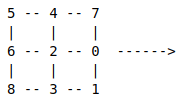
\includegraphics[width=38mm]{matriz-ini.png}
  }
  \subfigure{
  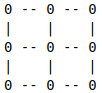
\includegraphics[width=22mm]{matriz-fin.png}
  }
  \caption{Reprersentación obtrención del valor mínimo red toroidal}
  \label{fig:toroide}
\end{figure}

\clearpage

\section{Diseño de la solución}
A continuación, se explicarán las funciones que forman parte del programa, el cual da una solución al enunciado de esta práctica.
\\

\subsection{Función principal del programa (\textit{main})}
Esta es la función principal del programa, en la cual como se puede observar lo primero que se lleva a cabo es la definicion de las variables a utilizar, como: \textit{rank}, \textit{numbers-n} (cantidad de números), \textit{size} (tamaño del toroide), \textit{data} (vector donde se almacenarán los números obtenidos del fichero), etc.

Tras esto se declarán las primitivas de \textit{\textbf{MPI}} como: 
\begin{itemize}
	\item \textit{MPI-Init}() \cite{mpi_init}: Para inicializar la estructura de comunicación de MPI entre los procesos. 
	\item \textit{MPI-Comm-Size}() \cite{mpi_size}: Para obtener el tamaño de la comunicacion (número de proceso a ejecutar en este caso, ranks), etc.
	\item \textit{MPI-Comm-rank}() \cite{mpi_rank}: Para establecer el identificador de cada proceso \textit{rank}.
\end{itemize}

También esta función se lleva a cabo las llamadas a las demás tipos de funciones que componen el programa

\lstinputlisting[language=C]{code/main.c}

\subsection{Lectura del fichero (\textit{load-data})}
La primera función a llamar dentro del \textit{main}, es la \textit{load-data()}, encargada de la lectura del fichero, esta función añade los números que almacena el fichero al vector de tipo \textit{long double} denominado \textit{data}.
Esta función obitiene los números del fichero, seprarando cada uno utilizando como separador la \textit{coma}.\\

Para la apertura del fichero se ha utilizado la función \textit{open-file()}, cuyo principal objetivo es devolver el descriptor del archivo \textit{datos.dat}.
A esta función se le pasa como parámetro \textit{DATA-PATH} que es la ruta del archivo a leer y \textit{READ-MOD} que indica el modo de apertura del archivo, en este caso el modo de lectura.
\lstinputlisting[language=C]{code/open_file.c}

Una vez cargados los datos en el vector \textit{data}, la función devolverá la variable \textit{i}, la cual almacena el valor de la cantidad de números que contiene el fichero.
\lstinputlisting[language=C]{code/load_data.c}

\subsection{Comprobación de la cantidad de números (\textit{check-size})}
Esta función se encarga de comprobar si la cantidad de números (\textit{numbers-n}) es igual al tamaño (\textit{size}) \cite{mpi_size} del toroide. Estos son los argumentos que se les pasa a la función.
La función devolverá True o False si es igual o no estas variables, si la devolución es False, entonces finalizará la ejecución normal del programa. Y el proceso \textit{rank 0}, mandará una difusión a los demás procesos, para que asi aborten su ejecución. Esto se realiza con la primitiva \textit{MPI-Bcast()} \citep{mpi_bcast}. 

\lstinputlisting[language=C]{code/bdcast.c}

\lstinputlisting[language=C]{code/check_size.c}


\subsection{Envio de su número a cada nodo (\textit{send-numbers})}
Esta función tiene el objetivo de añadir o enviar a cada nodo (\textit{rank}) \cite{mpi_rank} su número, esta tarea es realizada por\textit{rank 0}.

Tanto para el envio como para la recepción del nodo se han utilizado las primitivas basicas de MPI (\textit{MPI-Send \cite{mpi_send} y MPI-Recv \cite{mpi_recv}}).
Esta función recoge como parámetros el vector \textit{data} y la variable entera \textit{size} (tamaño toroide).

\lstinputlisting[language=C]{code/add_numbers.c}

Por último, se libera el espacio de memoria reservado para el vector de números \textit{data}.


\subsection{Obtención de los vecinos (\textit{get-neighbors})}
Esta función se encarga de que cada proceso, obtenga el rank de cada vecino, es decir, de sus vecinos \textit{Norte, Sur, Este y Oeste}. Para ello esta función recogerá como parámetros el rank del proceso que la ejecute, y su lista de vecinos vacía en este caso, representada mediante el vector de enteros llamado \textit{neighbors}.

Esta función es muy importante para la función que cálcula el mínimo número de la red toroidal \textit{calculate-min()}, debido que aquí cada nodo o rank conoce quienes son sus vecinos, con los cuales realizará dicha comprobaqción intgercambiando sus números.

El objetivo y funcionamiento de este algoritmo se ha explicado de una forma más teórica en el apartado 2, en concreto, la sección 2.2.1.

\lstinputlisting[language=C]{code/get_neighbors.c}

Como se puede observar el proceso de obtención se debide en dos partes, la obtención de los nodos pertenecientes a las filas y los pertenecientes a lo que serían las columnas.

\begin{itemize}
	\item \textbf{Filas}: por medio de las filas se obtienen los vecinos \textit{Norte} y \textit{Sur}, esto se realiza con la utilización de las fórmulas de la Tabla \ref{tab:filas}.
	\item \textbf{Columnas}: por medio de las columnas se obtienen los vecinos \textit{Este} y \textit{Oeste}, esto se realiza con la utilización de las fórmulas de la Tabla \ref{tab:columnas}.
\end{itemize}

La implementación en ambás partes se ha realizado con un \textit{switch}, en el cual dependiendo de la posición del \textit{rank} se obtrendrá de una forma u otra los vecinos.


\subsection{Cálculo del número mínimo (\textit{calculate-min})}
El objetivo principal de esta función es la del cálculo del número mínimo de la red toroidal completa, en el cual todos los elementos de la red deben de contener finalmente el número mínimo.

Para ello se explicará a continuaicón de una forma más práctica el procedimiento de este algoritmo, dado que en la sección 2.2.2 ya ha sido explicado de una forma más teoríca.

Por tanto, una vez obtenidos los vecinos de cada nodo, se lleva a cabo el cálculo del mínimo. 
La primera versión de este algoritmo estaba compuesta por dos bucles de tipo \textit{for}, en los cuales primero, se cálculaba los números de los vecinos correspondientes a las filas \textit{Norte y Sur}, enviando a \textit{Sur} el número que contiene el nodo actual y recibiendolo del \textit{Norte} su número. Y más tarde el mismo procedimiento con las columnas \textit{Este y Oeste}. Con cálcular me refiero a quedarse el nodo actual finalmente con el menor de cada número.
Para que esto sea aplicable a los elementos de toda la fila o de toda la columna se harían 1 a L-1 iteracciones en cada bucle.

Por lo que el procedimiento a seguir sería el siguiente:
\begin{itemize}
	\item \textbf{Primer bucle \textit{for}} (cálculo de las filas):
	\begin{enumerate}
		\item El \textit{rank} actual envía su número (\textit{my-number}) al vecino del \textit{Sur}.
		\item El \textit{rank} actual recibe el número de su vecino del \textit{Norte} (\textit{his-number}).
		\item Se realiza el cálculo del número mínimo entre estos dos número (se coge el menor de ellos).
	\end{enumerate}
	
	\item \textbf{Segundo bucle \textit{for}} (cálculo de las columnas):
	\begin{enumerate}
		\item El \textit{rank} actual envía su número (\textit{my-number}) al vecino del \textit{Este}.
		\item El \textit{rank} actual recibe el número de su vecino del \textit{Oeste} (\textit{his-number}).
		\item Se realiza el cálculo del número mínimo entre estos dos número (se coge el menor de ellos).
	\end{enumerate}
\end{itemize}

\lstinputlisting[language=C]{code/calculate-v1.c}


Como se puede observar, una vez realizado ambos bucles, todos los elementos de la red tendrán almacenado el número mínimo.


\subsubsection{Mejora del algoritmo}
Una vez desarrollada la primera versión del algoritmo de cálcular el mínimo, se observo, que realmente se realizaría lo mismo dejando simplemente un bucle \textit{for}, y además esto podría mejorar el rendmiento del programa.

El procedimiento de esta versión mejorada, es mas peculiar, debido a que no se calculan de forma secuencial, todos los vecinos de las filas (\textit{Norte-Sur}) y después los de las columnas \textit{Este-Oeste}, si no que cada nodo en una misma interacción calculará ambas opciones. El procedimiento a seguir sera el siguiente:

\textbf{En un único bucle \textit{for}}:
\begin{enumerate}
	\item El \textit{rank} actual envía su número (\textit{my-number}) al vecino del \textit{Sur}.
	\item El \textit{rank} actual recibe el número de su vecino del \textit{Norte} (\textit{his-number}).
	\item Se realiza el cálculo del número mínimo entre estos dos número, obtenidos de las filas (se coge el menor de ellos).
	\item El \textit{rank} actual envía su número (\textit{my-number}) al vecino del \textit{Este}.
	\item El \textit{rank} actual recibe el número de su vecino del \textit{Oeste} (\textit{his-number}).
	\item Se realiza el cálculo del número mínimo entre estos dos número, obtenidos de las columnas (se coge el menor de ellos).
\end{enumerate}

\lstinputlisting[language=C]{code/calculate_min.c}

Por último en ambas opciones, se libera el espacio de memoria reservado para el vector de los vecinos \textit{neighbors}.
\\

\subsubsection{Representación del flujo de eventos de envio y recepción}
Un ejemplo de representación del estado de la matriz, en un inicio y al final, este proceso se lleva a cabo en la función \textit{calculate-min()}, tras este proceso el resultado obtenido seria el siguiente:

\begin{figure}[H]
  \centering
  \subfigure{
    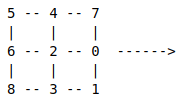
\includegraphics[width=38mm]{matriz-ini.png}
  }
  \subfigure{
  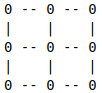
\includegraphics[width=22mm]{matriz-fin.png}
  }
  \caption{Representación red toroidal al inicio (izquerda) y al final (derecha)}
  \label{fig:toroide}
\end{figure}

Este proceso se lleva a cabo, como ya se ha explicado anteriormente gracías a un bucle \textit{for} que va de \textit{1} a \textit{(L - 1)}. A continuación, se mostrará de forma representativa (mediante una matriz que simulara la red toroidal), los cambios y pasos que sigue este proceso, desde su estado inicial al su estado final, se pueden ver en la Figura \ref{fig:toroide}. Caba destacar que el valor de la variable \textbf{\textit{L}} en este ejemplo es de \textbf{3}.

\begin{enumerate}
	\item \textbf{Estado inicial}
	\begin{figure}[H]
		\centering
		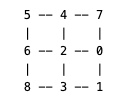
\includegraphics[width=30mm]{matriz-1.png}
		\label{fig:matriz-1}
	\end{figure}
	
	\item \textbf{Primera iteracción:} Cada \textbf{Rank} envía a su vecino \textit{Sur} su número y recibe el número de su vecino del \textit{Norte}. También cada \textit{Rank} enviará su número a su vecino \textit{Este} y recibirá el número del vecino del \textit{Oeste}. Entre medias de ambos procesos se calaculará el mínimo de cada cambio (explicado anteriormente en el apartado 4.6.1).
	\begin{figure}[H]
	\centering
	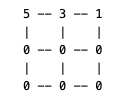
\includegraphics[width=30mm]{matriz-2.png}
	\label{fig:matriz-2}
	\end{figure}

	\item \textbf{Segunda iteracción:} Se realizarán de nuevo el mismo proceso que en la primera iteracción, debido a que así los ranks restantes tomen como número el valor mínimo. Este sería el \textbf{estado final del toroide}.
		\begin{figure}[H]
		\centering
		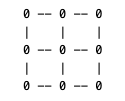
\includegraphics[width=30mm]{matriz-3.png}
		\label{fig:matriz-3}
		\end{figure}
	

\end{enumerate}







%%%%%%%%%%%%%%%%%%%%%%%%%%%%%%%%%%%%%%%%%%%%%%%%%%%%%%%%%%%%%%%%%%%%%%%%%%%%%%%%
%%%%%%%%% 						BIBLIOGRAFIA 						   %%%%%%%%%
%%%%%%%%%%%%%%%%%%%%%%%%%%%%%%%%%%%%%%%%%%%%%%%%%%%%%%%%%%%%%%%%%%%%%%%%%%%%%%%%
\newpage
\bibliography{biblist}
\bibliographystyle{plain}

%\nocite{*} Permite citar todas las referencias en el archivo .bib

% Añadir la bibliografía al Índice de contenidos
\ifspanish
	\addcontentsline{toc}{section}{Referencias}
\else
	\addcontentsline{toc}{section}{References}
\fi




\end{document}
